%% ----------------------------------------------------------------
%% Thesis.tex -- MAIN FILE (the one that you compile with LaTeX)
%% ---------------------------------------------------------------- 

% Set up the document
\documentclass[a4paper, 11pt, oneside]{Thesis}  % Use the "Thesis" style, based on the ECS Thesis style by Steve Gunn
\graphicspath{Figures/}  % Location of the graphics files (set up for graphics to be in PDF format)

% Include any extra LaTeX packages required
\usepackage[square, numbers, comma, sort&compress]{natbib}  % Use the "Natbib" style for the references in the Bibliography
\usepackage{verbatim}  % Needed for the "comment" environment to make LaTeX comments
\usepackage{vector}  % Allows "\bvec{}" and "\buvec{}" for "blackboard" style bold vectors in maths
\usepackage{graphicx}
\hypersetup{urlcolor=blue, colorlinks=true}  % Colours hyperlinks in blue, but this can be distracting if there are many links.
\setlength{\parindent}{4em}
\setlength{\parskip}{1em}
\usepackage{indentfirst}
\usepackage{threeparttable}
\usepackage{booktabs}
\usepackage{multirow}
\usepackage{bm}

%% ----------------------------------------------------------------
\begin{document}
\frontmatter      % Begin Roman style (i, ii, iii, iv...) page numbering

% Set up the Title Page
\title  {Long read error correction by short-read alignment using FM-index}
\authors  {\texorpdfstring
            {\textbf{{Yi-De Xie}}}
            {Yi-De Xie}
            }
\addresses  {\groupname\\\deptname\\\univname}  % Do not change this here, instead these must be set in the "Thesis.cls" file, please look through it instead
\date       {\today}
\subject    {}
\keywords   {}

\maketitle
%% ----------------------------------------------------------------

\setstretch{1.3}  % It is better to have smaller font and larger line spacing than the other way round

% Define the page headers using the FancyHdr package and set up for one-sided printing
\fancyhead{}  % Clears all page headers and footers
\rhead{\thepage}  % Sets the right side header to show the page number
\lhead{}  % Clears the left side page header

\pagestyle{fancy}  % Finally, use the "fancy" page style to implement the FancyHdr headers


%------------------


%------------------



%The Abstract Page
\addtotoc{Abstract}  % Add the "Abstract" page entry to the Contents
\abstract{
\addtocontents{toc}{\vspace{1em}}  % Add a gap in the Contents, for aesthetics
The third generation sequencing can generate multi-kilobase sequences and has the potential to improve genome assembly. Nevertheless, it has higher error rates in comparison with second generation sequencing. The error rates have limited its use to improve assembly. In this thesis, we introduce a hybrid correction algorithm to correct third-generation sequencing reads by finding overlapping short reads with high-quality. We improved the efficiency of a previous method which align short reads onto long PacBio reads using FM-index. The results indicate that the accuracy of corrected PacBio reads achieve over 93\%, the memory consumption is lower, and the running time is faster than previous method.

Keywords: Alignment, Second generation sequencing, Third generation sequencing
}

\clearpage  % Abstract ended, start a new page


%% ----------------------------------------------------------------

\setstretch{1.3}  % Reset the line-spacing to 1.3 for body text (if it has changed)

% The Acknowledgements page, for thanking everyone
%\acknowledgements{
%\addtocontents{toc}{\vspace{1em}}  % Add a gap in the Contents, for aesthetics

%The acknowledgements and the people to thank go here, don't forget to include your project advisor\ldots

%}
%\clearpage  % End of the Acknowledgements
%% ----------------------------------------------------------------

\pagestyle{fancy}  %The page style headers have been "empty" all this time, now use the "fancy" headers as defined before to bring them back


%% ----------------------------------------------------------------
%\lhead{\emph{Contents}}  % Set the left side page header to "Contents"
\tableofcontents  % Write out the Table of Contents


%% ----------------------------------------------------------------
%\lhead{\emph{List of Figures}}  % Set the left side page header to "List if Figures"
\listoffigures  % Write out the List of Figures

%% ----------------------------------------------------------------
%\lhead{\emph{List of Tables}}  % Set the left side page header to "List of Tables"
\listoftables  % Write out the List of Tables

%% ----------------------------------------------------------------
\setstretch{1.5}  % Set the line spacing to 1.5, this makes the following tables easier to read
%%\clearpage  % Start a new page
%%\lhead{\emph{Abbreviations}}  % Set the left side page header to "Abbreviations"
%%\listofsymbols{ll}  % Include a list of Abbreviations (a table of two columns)
%%{
% \textbf{Acronym} & \textbf{W}hat (it) \textbf{S}tands \textbf{F}or \\
%%\textbf{LAH} & \textbf{L}ist \textbf{A}bbreviations \textbf{H}ere \\

%%}


%% ----------------------------------------------------------------
% End of the pre-able, contents and lists of things
% Begin the Dedication page

\setstretch{1.3}  % Return the line spacing back to 1.3

%\pagestyle{empty}  % Page style needs to be empty for this page
%\dedicatory{For/Dedicated to/To my\ldots}

\addtocontents{toc}{\vspace{2em}}  % Add a gap in the Contents, for aesthetics


%% ----------------------------------------------------------------
\mainmatter	  % Begin normal, numeric (1,2,3...) page numbering
\pagestyle{fancy}  % Return the page headers back to the "fancy" style



% Include the chapters of the thesis, as separate files
% Just uncomment the lines as you write the chapters

\chapter{Introduction}


In recent years, next generation sequencing (NGS) technologies, including the 454 pyrosequencing~\cite{Marcel2005} in 2004 and Illumina sequencing-by-synthesis~\cite{Bentley2006}, have been widely used to sequence and assemble genomes of many species~\cite{NGS2010, genome10k2009}. NGS technologies, which have revolutionized DNA sequencing by diminishing cost and raising throughput, can yield $10^{8}$ short reads of length up to 200 bp with low error rates (2\%). 

%-> but the repetitive sequences may up to 1,300 bp
Regardless of benefit, NGS technologies still have several drawbacks. First, NGS technologies base on the Multiple Displacement Amplification (MDA) technology, leading to amplification artifacts~\cite{pmid24852006} and extremely non-uniform coverage of the genome~\cite{pmid21685062}. Secondly, because of the complex repeated sequences in genomes~\cite{pmid18341692}, the read length yielded by NGS are insufficient to cross the repeat region. For instance, the Illumina platforms generate reads up to 150 bp~\cite{pmid23644548} and the 454 sequencing yields reads of ~700 bp~\cite{pmid23644548} but the repetitive sequences may up to 1,300 bp~\cite{pmid25132181}. Therefore, numerous genomes sequenced and assembled by pure NGS are still too fragmented for subsequent analysis, such as gene annotation. 


Recently, the third generation sequencing (TGS) technology yields much longer reads in comparison with NGS. For example, the Pacific Biosciences (PacBio) sequencing technology generates reads up to ~20 kbp (average ~3 kbp)~\cite{pmid25705213}. In addition, because the entire sequencing protocol is single molecular, it requires no amplification and substantially reduces the sequencing bias~\cite{pmid20858600}. Hence, the longer reads make it useful for scaffolding de novo assemblies. Recently, the successful assembly of $E. coli K12$, $B. trehalosi$ and $M. haemolytica$ genomes have demonstrated the power of TGS~\cite{Koren2013}.

%Therefore-> Later
In reality, these TGS reads tend to have high error rates (up to 15\%) in comparison with NGS. On the basis of high-coverage PacBio sequencing, PBcR is able to self-correct the PacBio reads and assemble the genome. However, the cost of TGS is still very expensive, and high-coverage TGS is often not affordable in large genome sequencing projects. On the other hand, a few studies have been endeavoring to correct TGS reads using NGS reads. For example, the LoRDEC~\cite{Salmela2014} and the PacBioToCa~\cite{Koren2012}. The former uses bloom filters to build a de Bruijn graph that stands for NGS reads and corrects the erroneous region from corrective sequences in TGS reads by traversing the suitable paths in the graph. The latter corrects TGS reads individually by mapping NGS reads to them and computes high identity of hybrid consensus sequences. Later, TGS reads are able to be corrected by the NGS reads which aligns on TGS reads.


In this thesis, we introduce a error correction approach that utilizes NGS reads, high-identity sequences to correct TGS reads with the internal error. In particular, we use compressed data structures named FM-index~\cite{pmid20529929} that operate over a compressed representation of the full set of NGS reads since we require substantially lower the amount of memory to perform. Next, we align high-identity NGS reads on low-accuracy TGS reads and in our expectation, TGS reads can be modified based on the information from aligned NGS reads. Eventually, the corrected TGS reads would have much lower error rates than original TGS reads. As demonstrated below for several genomes, including 4.6 Mbp genome size of $Escherichia coli K12$ and 100.2 Mbp genome size of $C elegans$, we will evaluate the performance according to the yield (the number of TGS read aligned on reference genome after correction), accuracy rates after correction, memory usage, and the running time for each species by each software which we mentioned above and our method. % Introduction

\chapter{Literature Review}

\section{Next Generation Sequencing}

Over the past few years, there has been a fundamental change from the Sanger sequencing in genome analysis\cite{Maxam1977,Sanger1977}. Prior to this departure, the Sanger sequencing had dominated the industry for almost twenty years and led to many significant accomplishments, including the completion of the only finished-grade human genome sequence\cite{HGP2004}. In spite of many technical improvements during this era, the limitations of Sanger sequencing showed a demand for new and improved technologies for sequencing large numbers of human genomes. Development of new methods has been a new target to achieve, leaving Sanger sequencing with fewer reported advances. The Sanger sequencing is considered as a 'first-generation' technology, and newer methods are referred to as next-generation sequencing (NGS)\cite{Mardis2008}. These newer technologies involve various strategies that rely on a combination of template preparation, sequencing and imaging, and genome alignment and assembly methods. The arrival of NGS technologies has changed the way we think about scientific approaches and clinical research in basic. The ability to produce an enormous volume of data cheaply is the major advance offered by NGS - in some cases more than one billion short reads per cyclic run\cite{Wheeler2008}. Determining the order of bases is not the only thing to be considered for the reason that the feature of NGS expands the realm of experimentation. The ability to sequence the whole genome of many individuals in a population has allowed large-scale comparative and evolutionary studies to be implemented that were unimaginable just a few years ago. Here, we will present a technical review of template preparation to provide guidance on how these technologies work.

\section{Third Generation Sequencing}
Third-generation sequencing has two main characteristics comparison with the next generation sequencing~\cite{pmid22829749}. First, PCR isn't needed before sequencing, which shortens DNA preparation time for sequencing. Second, the signal is captured in real time so that the signal is monitored during the enzymatic reaction. For example, Pacific Bioscience released their first commercial third-generation sequencing instrument, PacBio RS: a real-time, single-molecule sequencer. It takes 4 to 6 hours instead of days to prepare the sample and it also does not need PCR step in preparation step, which reduces the bias and error caused by PCR. Furthermore, the average read length is up to 1300 bp, which is longer than second-generation sequencing technology. These technologies are quite useful for $de novo$ genome and transcriptome assembly as they have the potentail to resolve complex repeats and span entire gene transcripts. However, this instrument generates reads that average only $82.1\%-84.6\%$~\cite{pmid21142692, pmid21793740} nucleotide accuracy, with uniformly distributed errors dominated by point insertions and deletions~\cite{Koren2012}. This high error rates obscures the alignments between reads and complicates analysis since the pairwise differences between two reads is approximately twice their individual error rates, and is far beyond the $5\%–10\%$ error rates~\cite{Marcel2005, pmid18952627, pmid22147368} that most genome assemblers can tolerate—simply increasing the alignment sensitivity of traditional assemblers is computationally infeasible. Additionally, the PacBio technology utilizes hairpin adaptors for sequencing double stranded DNA, which can result in chimeric reads if the sequencing reaction processes both strands of the DNA (first in the forward and then reverse direction). While it is possible to generate accurate sequences on the PacBio RS by reading a circularized molecule multiple times (circular consensus or CCS), this approach reduces read length by a factor equal to the number of times the molecule is traversed, resulting in much shorter reads (e.g. median = 423 bp, max= 1,915 bp). Thus, there is a great potential advantage to the long, single-pass reads if the error rates can be algorithmically managed~\cite{Koren2012}.


\section{Sequencing error}
A sequencing error or mis-call occurs when a sequencing method calls one or more bases incorrectly, leading to an inaccurate read. Due to the vagaries of molecular biology, no laboratory-based DNA sequencing methods are perfectly precise; they are all known to mis-call bases occasionally in the machines. The chance of a sequencing error is generally known and quantifiable, thanks to extensive testing and calibration of the sequencing machines. Each base in a read is assigned a quality score, indicating confidence that the base has been called correctly. Some sequencing methods are more reliable than others and so give higher quality scores. Sequencing errors are also more likely to appear at the end of a read, far from where the insert has begun, so quality scores there are typically lower~\cite{sequencing_error}.

\subsection{Types of sequencing errors}
\begin{description}

\item [Mismatch.]
A mismatch is a substitution of one base for another, e.g., an A for a C. Mismatches are different from SNPs, which are actual differences in the genome (due to polymorphism). It is not easy to distinguish mismatches from SNPs, especially at low coverage. Mismatches are often fixed during error correction.

\item [Indel.]
An indel, short for "insertion/deletion", occurs when a read contains a different number of bases from its reference at some points in the alignment. An insertion occurs when the read contains extra bases, while a deletion occurs when the read is missing bases. Indels, like mismatches, may actually be true indicators of polymorphism rather than the result of sequencing errors.
\end{description}

\section{FM-index}
In computer science, an FM-index is a compressed full-text substring index based on the Burrows-Wheeler transform, with some similarities to the suffix array. It was created by Paolo Ferragina and Giovanni Manzini~\cite{Ferragina2000}, who describe it as an opportunistic data structure as it allows compression of the input text while still permitting fast substring queries. The name stands for Full-text index in Minute space~\cite{Ferragina2005}.It can be used to efficiently find the number of occurrences of a pattern within the compressed text, as well as locate the position of each occurrence. Both the query time and storage space requirements are sublinear with respect to the size of the input data. The original authors have devised improvements to their original approach and dubbed it "FM-Index version 2". A further improvement, the alphabet-friendly FM-index, combines the use of compression boosting and wavelet trees~\cite{Ferragina2004} to significantly reduce the space usage for large alphabets~\cite{wiki:FM-index}. The FM-index has found use in, among other places, bioinformatics~\cite{pmid20529929}. % Background Theory 

\chapter{Method}

\section{Overview}

%seed identification-> short reads collection
The error correction algorithm first collects short reads having the same seed (substrings of length $k$) with each PacBio read. These short reads are aligned onto the PacBio read using a hit-and-extend strategy in conjunction with banded dynamic programming. The errors in each PacBio read, including insertions, deletions, and mismatches, are then replaced with the major alleles in the aligned short reads. In practice, the running time of the above algorithm is unacceptable due to the long length of PacBio reads and huge amount of short reads. The time complexity of each step is listed in Figure~\ref{correction_process}. The following Figure~\ref{correction_process} demonstrates the entire flow of our method, including short reads collection using FM-index, extraction of read sequence, banded dynamic programing, and correction.

\newpage % Overview ended, start a new page to fill figure
\begin{figure}
\centering
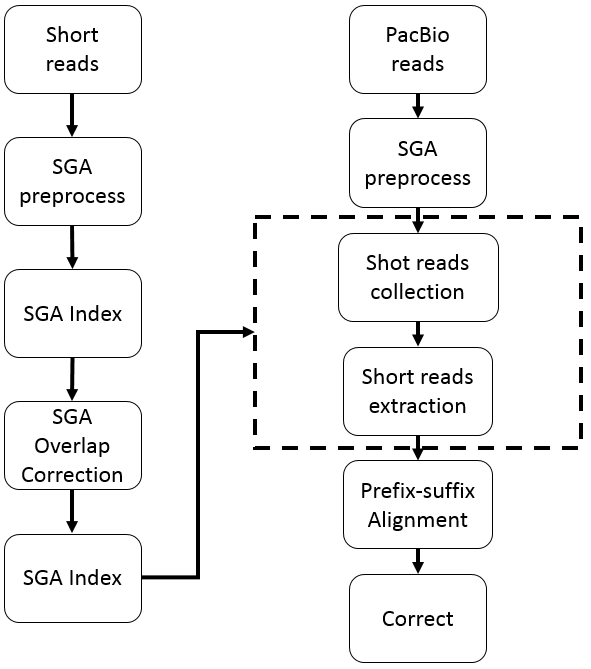
\includegraphics[scale=0.50]{Figures/chapter3/correction_process.png}
\caption{Error correction process}
\label{correction_process}
\end{figure}

\section{Short Reads Collection Using FM-index}


The FM-index of short reads was constructed using Li's ropebwt2 algorithm~\cite{pmid25107872}. Only the short reads sharing common $k$-mer with PacBio reads, which named seed, are considered for correction. The collection of common seeds is done by sliding a $k$-mer window (19 bp by default) along the entire PacBio read. For each $k$-mer in a window, the corresponding suffix array (SA) interval in BWT is computed using the backward search algorithm~\cite{pmid20529929}. In reality, the SA interval within repeats can be very large, and the extraction of each SA index within a repeat interval is extremely slow and less sensitive. In order to reduce the running time, the intervals of per $k$-mer are limited to constant value, which might change due to the coverage, leading to $O(CRk)$ time complexity, where $C$ is the upper limit of SA indices sampled from each SA interval, $R$ is the length of PacBio read and $k$ is the length of a $k$-mer. In our program, $C$ is a used-provided parameter relative to the sequencing coverage. 

\begin{figure} [h]
\centering
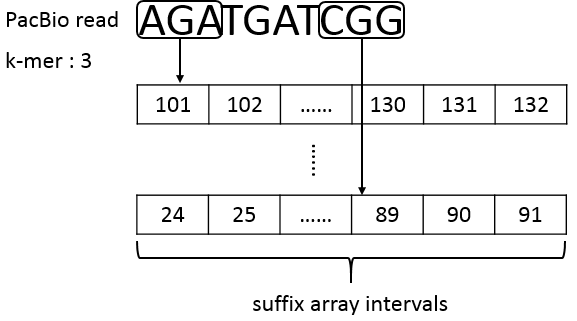
\includegraphics[scale=0.45]{Figures/chapter3/seed_identification.png}
\caption{Example of Short Reads Collection}
\label{Seed_Identification}
\end{figure}


\section{Extraction of Read Sequences from FM-index}

%seed identified-> short reads collected
Each short read having common seed with the PacBio read will be used for correction. However, the short reads collected in previous step only provide implicit SA intervals instead of explicit read sequences, which are required in subsequent pairwise dynamic programming. Therefore, each SA index within the interval needs to be first converted to corresponding read sequence using LF-mapping algorithm~\cite{pmid19261174}. Note that each SA index implies a suffix position within a read. The algorithm has to first backtract from any position to the ending position of the corresponding read (via LF-mapping), and then the sequence can be reconstructed by backtracting from the ending position to the starting position~\cite{pmid20529929}. By assumming the seeds are uniformly distributed in the PacBio read, the expected running time of above algorithm would be $1.5r$, where $r$ is the length of short read.

In order to reduce the time required for backtracting the entire read, we loaded the entire read sequences into memory, which are indexed by read IDs. The above algorithm can thus terminate immediately when backtracting from any suffix position to the ending position, where the read ID can be known and the read sequence can be obtained immediately. This reduces the expected running time from $1.5r$ to $0.5r$, if seeds are uniformly distributed in a PacBio read. Although the entire time complexity is still $O(CRr)$.

\begin{figure} [h]
\centering
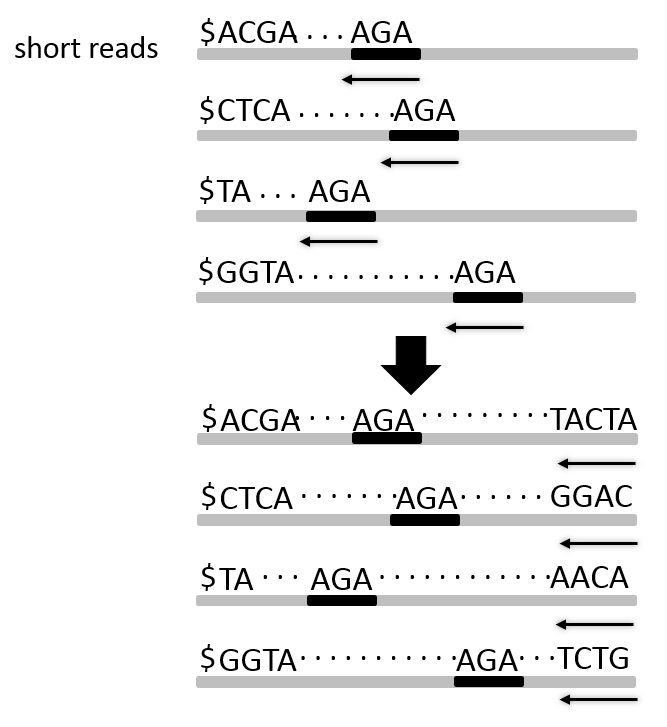
\includegraphics[scale=0.50]{Figures/chapter3/extraction_fm_index.png}
\caption{Extraction by FM-index}
\label{extraction_fm_index}
\end{figure}

\begin{figure} [h]
\centering
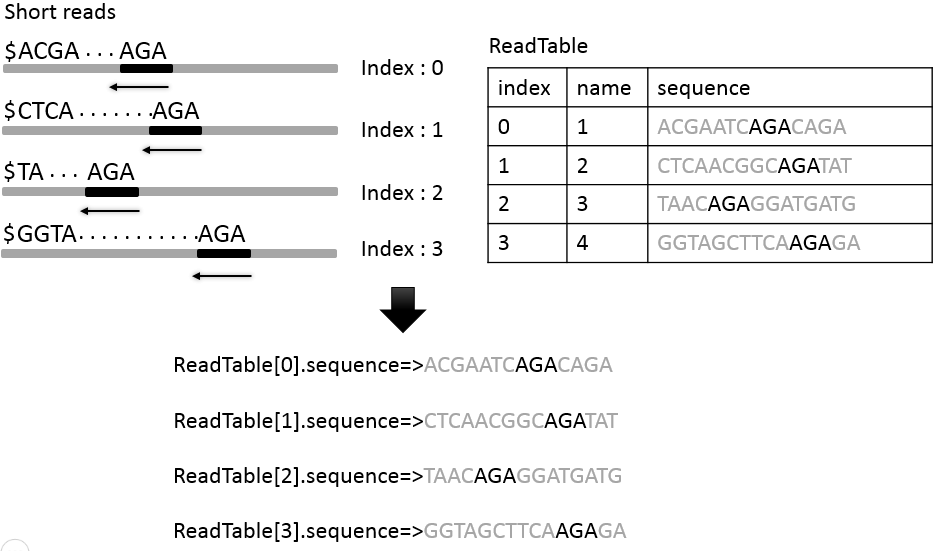
\includegraphics[scale=0.5]{Figures/chapter3/extraction_readtable.png}
\caption{Extraction by readtable}
\label{extraction_readtable}
\end{figure}

\newpage

\section{Prefix-suffix Alignment Using Banded Dynamic Programing}

Each read sequence extracted in previous step is aligned against the PacBio read (sharing common seeds). However, as the PacBio read is rather long ($R>>r$), the original dynamic programming for both reads is rather time-consuming ($O(Rr)$). Because each short read can only be aligned to a small fraction of the PacBio read, the dynamic programming can be further restricted into a smaller fraction surrounding the seed. 


In particular,the total number of insertions and deletions in the alignment is limited to $d-1$ (20 bp by default). Therefore, the alignment should be within the $(d)$ bandwidth centered at the seeding region, and it is unnecessary to compute the lower and upper triangles with respect to the seeding region. We estimate the necessary regions for dynamic programming according to the seed starting positions in PacBio ($P$) and short reads ($p$). The tabular computation can be restricted to $(P-p, P-p+r)$, where $P \geq p$. As a result, the best score of prefix-suffix alignment between these two reads ($S_{i,j}$, where $0 \leq i \leq r$ and $(P-p) \leq j \leq (P-p+r) $) can be computed using the following banded dynamic programming (See figure~\ref{banded_DP_table_with_d3}).
 %or $(0, r-(p-P))$, where $P < p$

\vspace{6pt}
$S_{i,j} = \max \left\{\begin{matrix} S_{i-1, j} - 3 &, insertion\\
S_{i, j-1} - 3 &, deletion\\
S_{i-1, j-1} - 5 &, mismatch\\
S_{i-1, j-1} + 8 &, match \end{matrix}\right\}, 0 \leq i \leq r, (P-p) \leq j \leq (P-p+r)$ 

After finishing the banded DP, we start to trace back at the position $max_{i,j}S(i,j)$ and redo the calculations in the backwards direction to find out where the score came. In other words, from the position $max_{i,j}S(i,j)$, we recalculate $S(i-1,j)$ which is deletion, $S(i-1,j-1)$ which is match or mismatch, and $S(i,j-1)$ which is insertion until the the beginning of baned DP. With the recalculate, we can reconstruct the path that may be with match, mismatch, insertion, deletion (See figure~\ref{Traceback_DP}).


%% This is so confusing. The complexity looks sometimes is all PacBio reads and sometimes only one PacBio read. What exactly are you computing?
For time analysis, note that the area of the $d$ band in the table is $rd$ and the time for filling in every entry inside the band is $O(1)$. In traceback step, the length of the path is approximately $r$ and the time for recalculating in every entry in the path is $O(1)$. Hence, the running time of banded DP algorithm is $O(CRrd)$.

\begin{figure} [h]
\centering
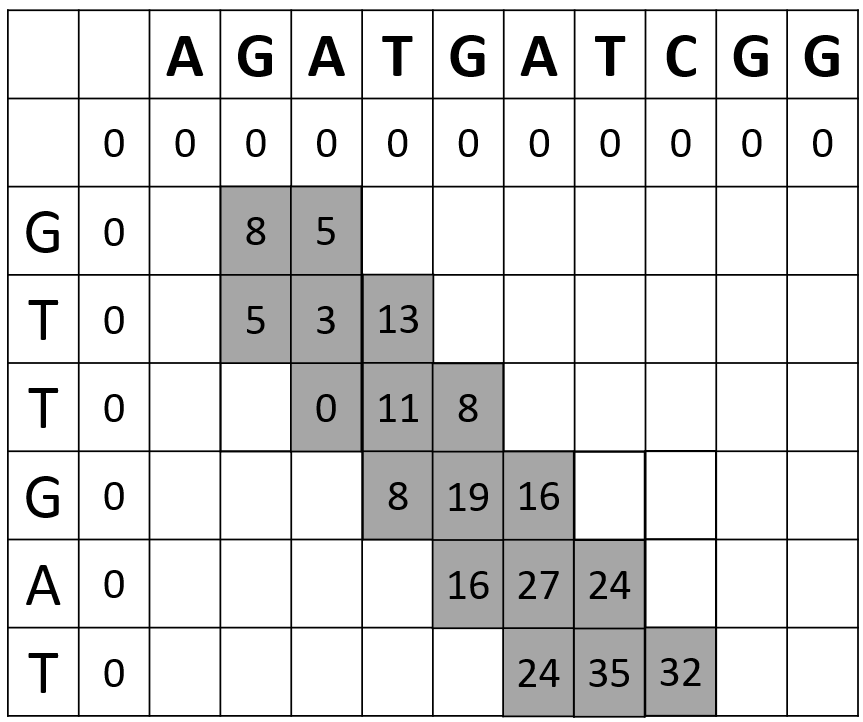
\includegraphics[scale=0.35]{Figures/chapter3/banded_DP_table_with_d3.png}
\caption{An example for banded dynamic programming table with $d=3$}
\label{banded_DP_table_with_d3}
\end{figure}

\begin{figure} [h]
\centering
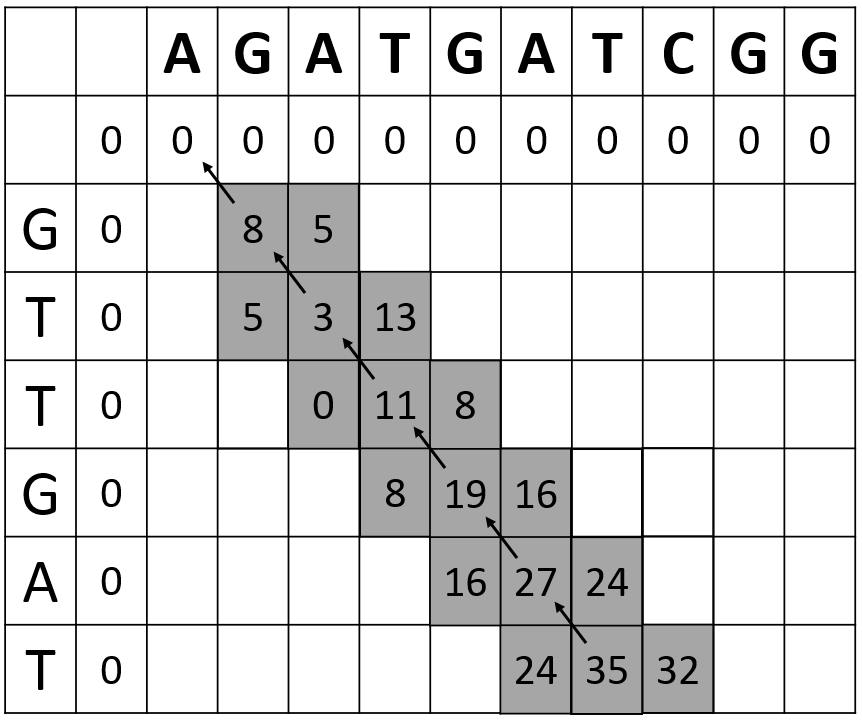
\includegraphics[scale=0.35]{Figures/chapter3/Traceback_DP.png}
\caption{Traceback of banded dynamic programming}
\label{Traceback_DP}
\end{figure}

\newpage

\section{Replacement of Errors by Major Allele}

At this stage, the alleles $(A, T, C, G, -)$ aligned to each base of the PacBio read are known. And the erroneous PacBio allele is replaced with the most-frequent allele (See figure~\ref{replacment}). In reality, there may exist two or more alleles both with high frequencies, owing to SNPs or repeat alleles. If PacBio allele is among the the highest frequency ones, it is retained. Otherwise, it is replaced with arbitrary highest-frequent alleles (if more than one).


Below, we analyze the time complexity of the correction. The time of statistics is $O(CRr)$, where $CR$ is the number of short reads and $r$ is the length of short read. For the replacement, it has to take $O(R)$ to check every position of the PacBio read and extracts elements of each position is $O(1)$. Totally, the time complexity of correction is $O(CRr+R)$

\begin{figure} [h]
\centering
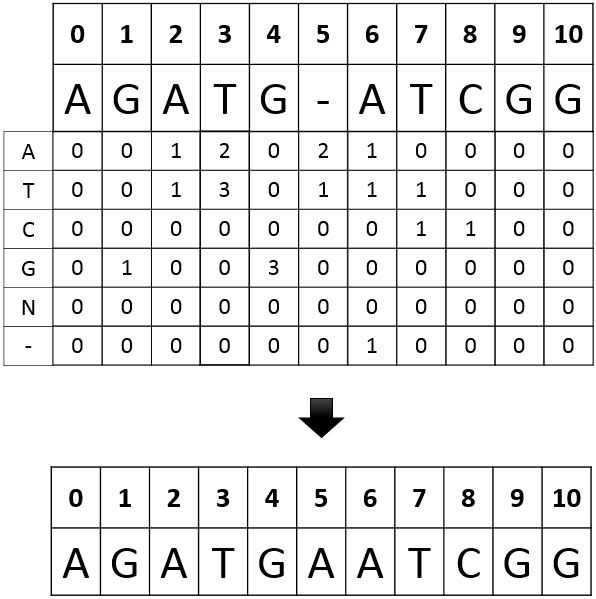
\includegraphics[scale=0.5]{Figures/chapter3/replacmentOfcorrection.png}
\caption{An example of Replacement of Errors by Major Allele}
\label{replacment}
\end{figure}

\newpage

\section{Parallelization}

We tried three parallelization methods including pthread, openMP, and an division-based method in conjunction with openMP. The first is based on Mutex that it will process the thread-number PacBio reads at once time and wait until all threads are finished. In practice, the length of PacBio reads are not uniform so that the running time of processing for each PacBio read is various. The numbers of procedures would wait until the slowest procedure completed at a time. The second separate the procedure into three distinct parts, Reading data from the file, Processing data, and Writing data into the file. Therefore, we have to set critical section lock Reading data from the file and Writing data into the file to avoid race condition and we barely parallel Processing data. In reality, it take too much overhead on critical section, as a result, we figure out the third method that is also based on openMP. Divided-file openMP separates equally the input file and the output file into the numbers of threads. For each thread, it has its own files, which is a input file and a output file, and consequently, we are able to parallel the procedure from reading data to writing data.

\begin{figure} [h]
\centering
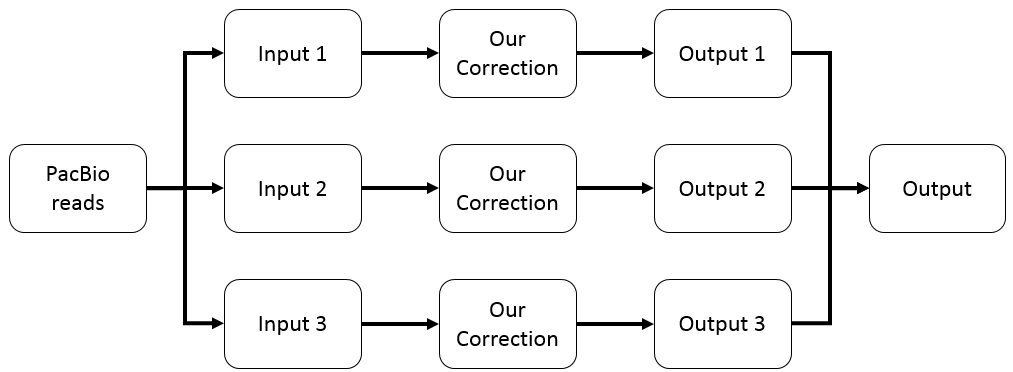
\includegraphics[scale=0.4]{Figures/chapter3/divided_file_openMP.png}
\caption{An example of Divided-file openMP with thread = 3}
\label{divided_file_openMP}
\end{figure} % Method

\chapter{Material and Results}

\section{Comparison of time complexity and running time}


In this paragraph, we summarized the time complexity of each step of our correction in comparison with SGA correction in figure~\ref{timecomplexity}. The major differences between our correction and SGA correction are steps 3 and 4. In step 3, we improved the time complexity from $O(CR^{2}d)$ to $O(CRrd)$, where $R>>r$. In reality, $R$ is roughly ranges from 4000 bp to 16,000 bp, and $r$ is equivalent to ~100bp. In step 4, the time complexity is improved from $O(CR^2)$ to $O(CRr)$.

We sampled ten PacBio reads from real data of $C elegans$ and investigated the real running time of the four steps (see Figure~\ref{timecomplexityonrealdata}). The running time of step 3 improves significantly and that of step 4 slightly improves in comparison with those of original SGA correction. 

\newpage

\begin{figure} [h]
\centering
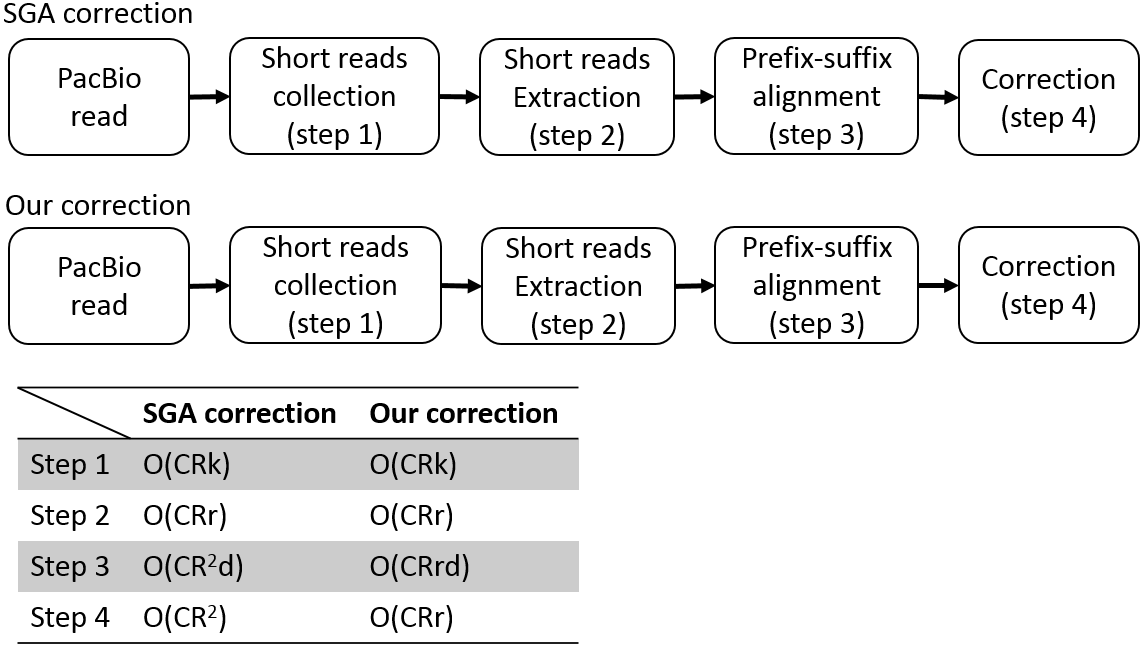
\includegraphics[scale=0.45]{Figures/chapter4/timecomplexity.png}
\caption{The time complexity of SGA correction and our correction}
\label{timecomplexity}
\end{figure}

\begin{figure} [h]
\centering
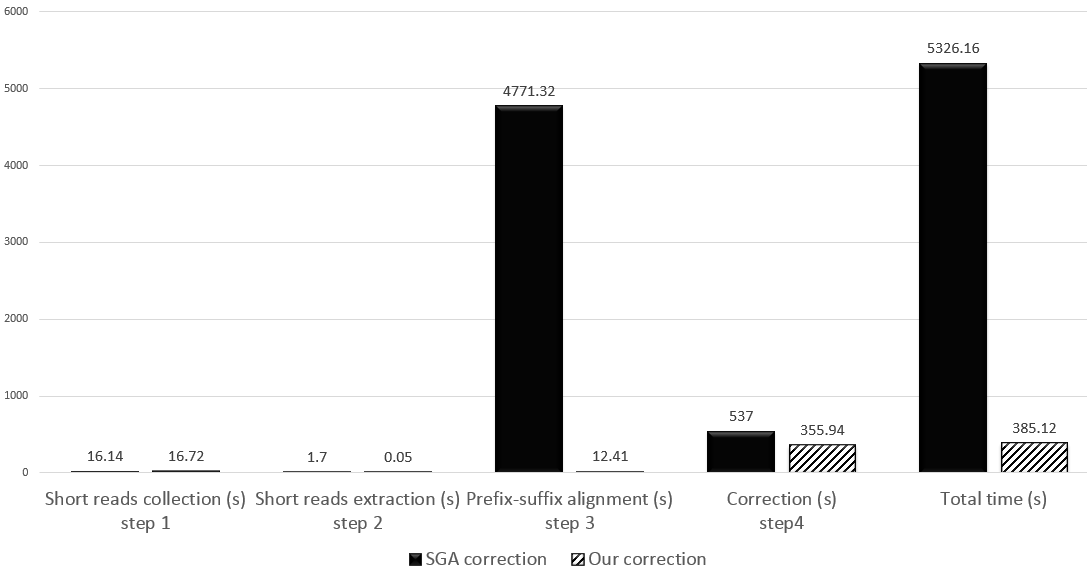
\includegraphics[scale=0.5]{Figures/chapter4/timecomplexityonRealdata.png}
\caption{Comparison of the real running time with SGA correction for each step}
\label{timecomplexityonrealdata}
\end{figure}

\section{Material}

We used three data sets composed of both short reads (from Illumina sequencing) and PacBio reads (from PacBio sequencing) to assess our correction (see Table~\ref{thedataset}). The first two data sets are from the same $E coli.$ strain, where the PacBio read length differs a lot owing to usage of old and new chemistry. The third data set contains both Illumina and PacBio sequencing reads from a larger genome $C. elegans$.
%The average length of the first \textit{E.coli} dataset is 3,981 bp, the maximum length is 14,494 bp and the coverage is 20 times. 
%The average length of the second dataset is 13,660 bp, the maximum length is approximately 50,000 bp, and the coverage is 140 times. 
%The average length of sampled \textit{C elegans} is 16,718 bp. The datasets was performed by SGA overlap correction, PacBioToCA, and our correction.

\newpage

\section{Results on the First Data Set}
%many seeds with frequency-> many short reads with frequency of k-mer
%sample seeds-> samples short reads
In the first data set, the running time of SGA correction is faster than our method (Table~\ref{resultOffirstDataset}), whereas PacBioToCA is the slowest. In terms of accuracy, PacBioToCA is higher than ours, whereas SGA is the lowest. The running time of our method didn't outperform SGA as expected, which is due to the ultra high coverage of Illumina sequencing. SGA gives up many short reads with frequency of $k$-mer larger than 200, while our method uniformly samples short reads across the entire PacBio read. Therefore, although SGA gains speed, it sacrifices accuracy in comparison with our method. In addition, the PacBio reads are relatively shorter (i.e., ~4000bp owing to usage of earlier chemistry), and the performance improvement of our method is not significant.

\section{Results on the Second Data Set}

In the second data set, the PacBio reads are much longer and sequencing coverage are relatively lower compared with the first data set. Table~\ref{resultOfsecondDataset} lists the running time and accuracy of corrected PacBio reads. The results indicate that our method is the fastest, SGA is the second, and PacBioToCA is the slowset. In terms of accuracy, PacBioToCA is still the highest, our method is the second, and SGA is the lowest. The speedup of our method compared with SGA can be revealed in this data set owing to longer PacBio read and lower Illumina sequencing coverage. 

\section{Results on the Third Data Set}
%PacBioToCA still can't finish by the time of writing this manuscript-> PacBioToCA continued to correct PacBio reads for four days but it still can't finish
In the third data set, all programs can not finish execution within a reasonable period of time and we down-sample the PacBio reads to 4,790. PacBioToCA continued to correct PacBio reads for four days but it still can't finish. The results indicate our method is much more efficient than SGA (Table~\ref{resultOfthirdDataset}). This is due to an ordinary Illumina sequencing coverage and much longer PacBio reads of this data set. And the accuracy of our method is higher than that of SGA. 

\newpage

\begin{table}[h]
\centering
\caption{The datasets}
\label{thedataset}
\resizebox{\textwidth}{!}{%
\begin{tabular}{@{}lrrrrr@{}}
\toprule
\textbf{} & \textbf{Average length (bp)} & \textbf{Maximum length (bp)} & \textbf{Number of read} & \textbf{Sequencing throughput (bp)} & \textbf{Coverage} \\ \midrule
The first set of E.coli \\
PacBio reads & 3,981 & 14,494 & 35,161 & 94.3 M & 20.5  \\
Short reads & 102 & 102 & 44.8 M & 4,531 M & 985 \\ \midrule
The second set of E.coli \\
PacBio reads & 13,660 & 49,424 & 144,960 & 644 M & 140 \\
Short reads & 100  & 100  & 28.4 M & 2,840 M & 617  \\ \midrule
C elegans \\
PacBio reads & 16,591 & 44,883 & 4,790 & 51 M & 0.5\\ 
Short reads reads & 110  & 110  & 133 M & 14,640 M & 146 \\ \bottomrule
\end{tabular}
}
\end{table}

\begin{table}[h]
\centering
\caption{The comparison of the performance and the accuracy for the first dataset of E.coli}
\label{resultOffirstDataset}
\resizebox{\textwidth}{!}{%
\begin{tabular}{@{}lrrrr@{}}
\toprule
\textbf{} & \textbf{Raw data} & \textbf{PacBioToCA} & \textbf{SGA correction} & \textbf{My correction} \\ \midrule
Running time (hour) & - & 33.41 & 0.33 & 1.33 \\ 
Peak memory usage (Mb) & - & 74,279 & 1,055 & 11,949 \\ 
Number of read & 35,161 & 107,409 & 35,161 & 35,161 \\
Number of PacBio read aligned on reference & 31,971 & 107,283 & 31,971 & 31,990 \\ 
Identity (\%) & 83.57 & 99.83 & 87.01 & 93.23 \\
Average length (bp) & 4,083 & 1,536 & 4,029 & 4,037 \\
Maximum length (bp) & 14,494 & 10,925 & 14,452 & 14,452 \\ \bottomrule
\end{tabular}
}
\end{table}

\begin{table}[h]
\centering
\caption{The comparison of the performance and the accuracy for the second dataset of E.coli}
\label{resultOfsecondDataset}
\resizebox{\textwidth}{!}{%
\begin{tabular}{@{}lrrrr@{}}
\toprule
\textbf{} & \textbf{Raw data} & \textbf{PacBioToCA} & \textbf{SGA correction} & \textbf{My correction} \\ \midrule
Running time (hour) & - & 44 & 9 & 5.5 \\ 
Peak memory usage (Mb) & - & 156,212 & 628 & 6,782 \\ 
Number of read & 144,960 & 427,109 & 144,960 & 144,960 \\
Number of PacBio read aligned on reference & 48,207 & 427,007 & 48,223 & 49,750 \\
Identity (\%) & 84.58 & 99.87 & 84.98 & 94.30 \\
Average length (bp) & 13,660 & 3,360 & 13,635 & 13,660 \\
Maximum length (bp) & 20,749 & 25,709 & 20,722 & 20,749 \\ \bottomrule
\end{tabular}
}
\end{table}

%\begin{table}[h]
%\centering
%\begin{threeparttable} 
%\caption{The comparison of the performance and the accuracy for C elegans}
%\label{resultOfthirdDataset}
%\resizebox{\textwidth}{!}{%
%\begin{tabular}{@{}lrrrr@{}}
%\toprule
%\textbf{} & \textbf{Raw data} & \textbf{PacBioToCA} \tnote{a} & \textbf{SGA correction} & \textbf{My correction} \\ \midrule
%Runnin time (hour) & - & - & 19.10 & 0.75 \\ 
%Memory usage (Mb) & - & - & 3,311 & 31,732 \\ 
%Number of read & 4,790 & - & 4,790 & 4,790 \\
%Number of PacBio read aligned on reference & 4,729 & - & 4,729 & 4,731 \\ 
%Identity (\%) & 87.81 & - & 87.90 & 96.38 \\
%Average length (bp) & 16,591 & - & 16,572 & 16,521 \\
%Maximun length (bp) & 44,883 & - & 44,833 & 44,841 \\
%\end{tabular}
%\begin{tablenotes}  
%\item[a] 123
%\end{tablenotes} 
%}
%\end{threeparttable} 
%\end{table}

%\begin{document}

\begin{table}[htbp]  
\centering  
\begin{threeparttable}
\caption{The comparison of the performance and the accuracy for C elegans}  
{
\label{resultOfthirdDataset}
\scriptsize 
\setlength\tabcolsep{3pt} 
\begin{tabular}{@{}lrrrr@{}}
\toprule
\textbf{} & \textbf{Raw data} & \tnote{*} \textbf{PacBioToCA} & \textbf{SGA correction} & \textbf{My correction} \\ \midrule
Running time (hour) & - & - & 19.10 & 0.75 \\ 
Peak memory usage (Mb) & - & - & 3,311 & 31,732 \\ 
Number of read & 4,790 & - & 4,790 & 4,790 \\
Number of PacBio read aligned on reference & 4,729 & - & 4,729 & 4,731 \\ 
Identity (\%) & 87.81 & - & 87.90 & 96.38 \\
Average length (bp) & 16,591 & - & 16,572 & 16,521 \\
Maximum length (bp) & 44,883 & - & 44,833 & 44,841 \\ \bottomrule
\end{tabular}   
\begin{tablenotes}  
\item[*] Comparison with other methods, it took too much time (up to four days) so it's not necessary to finish it.
\end{tablenotes}  
}  
\end{threeparttable}  
\end{table}  

%\end{document} % Results and Discussion

\chapter{Conclusion and Future Works}

\section{Summary}
PacBio reads have the advantage of scaffolding de novo assemblies but they usually have high error rate. Before making use of PacBio reads, it is important to correct them. In this study, we improved the performance and accuracy of SGA correction for PacBio reads. Our correction filtered out short reads sharing common $k$-mer with PacBio reads from total short reads, aligned short reads on PacBio reads, which used banded dynamic programming, and replaced errors of PacBio reads by major allele. The experimental results showed that Our correction is faster than SGA correction and PacBioToCA, which also correct PacBio reads by alignment, according to the average length of PacBio reads. Besides, our correction has higher accuracies than raw data and SGA correction.

\section{Future Works}
In this section, we propose some possible directions for future research. After we improved the performance of SGA correction, there are still some sequencing errors, which were not mentioned previously. For instance, chimera reads~\cite{Koren2012}. This may cause misassemblies so solving this error has the higher priority in the future research. % Conclusion

%\chapter{Material and Results}

\section{Comparison of time complexity and running time}


In this paragraph, we summarized the time complexity of each step of our correction in comparison with SGA correction in figure~\ref{timecomplexity}. The major differences between our correction and SGA correction are steps 3 and 4. In step 3, we improved the time complexity from $O(CR^{2}d)$ to $O(CRrd)$, where $R>>r$. In reality, $R$ is roughly ranges from 4000 bp to 16,000 bp, and $r$ is equivalent to ~100bp. In step 4, the time complexity is improved from $O(CR^2)$ to $O(CRr)$.

We sampled ten PacBio reads from real data of $C elegans$ and investigated the real running time of the four steps (see Figure~\ref{timecomplexityonrealdata}). The running time of step 3 improves significantly and that of step 4 slightly improves in comparison with those of original SGA correction. 

\newpage

\begin{figure} [h]
\centering
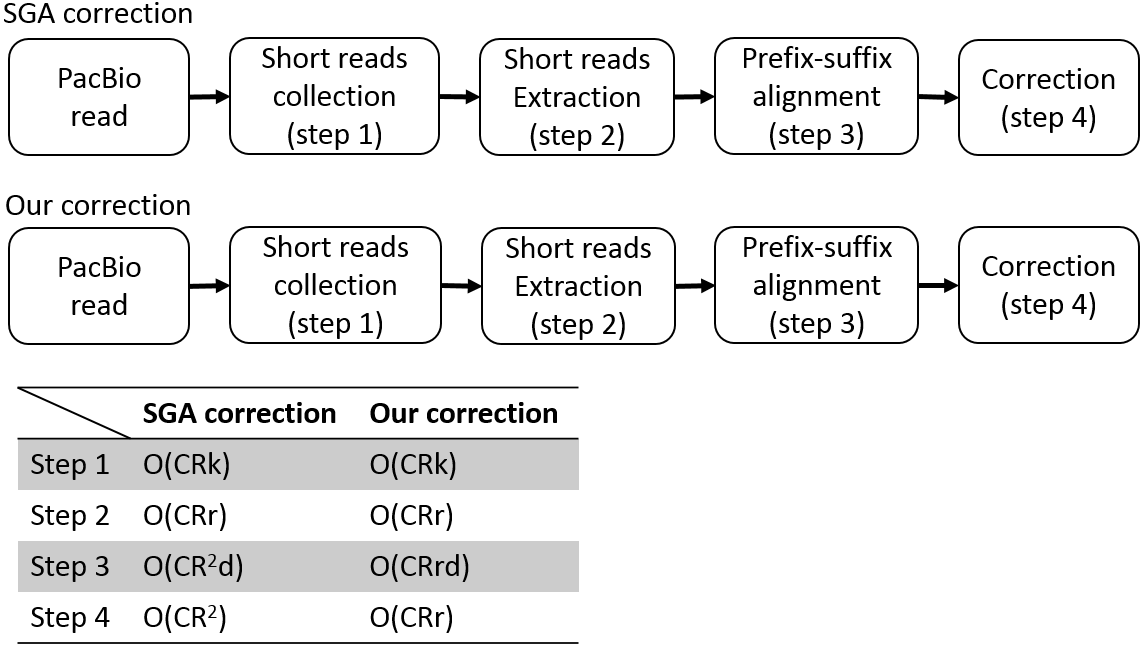
\includegraphics[scale=0.45]{Figures/chapter4/timecomplexity.png}
\caption{The time complexity of SGA correction and our correction}
\label{timecomplexity}
\end{figure}

\begin{figure} [h]
\centering
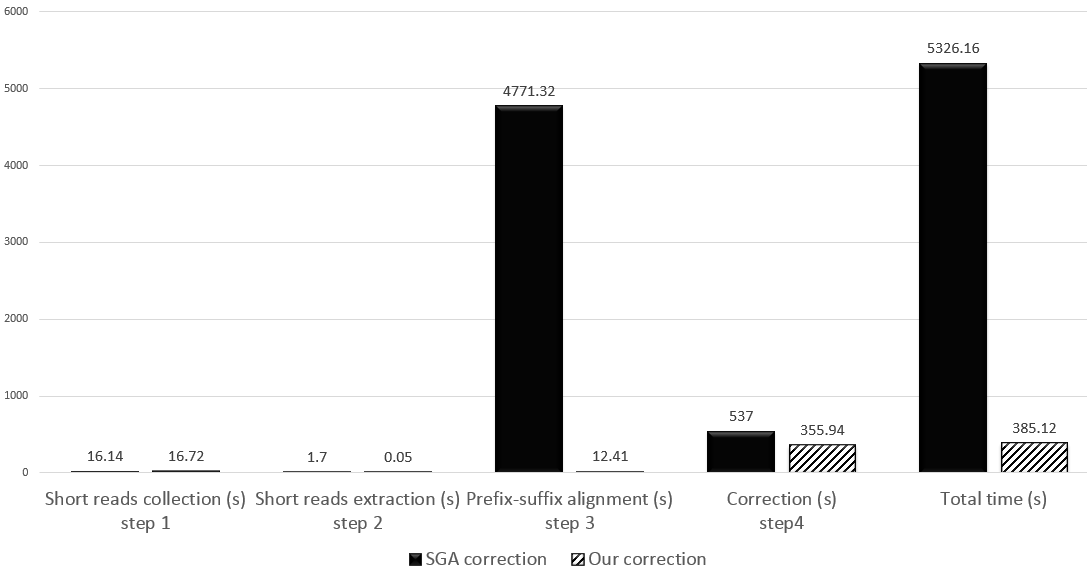
\includegraphics[scale=0.5]{Figures/chapter4/timecomplexityonRealdata.png}
\caption{Comparison of the real running time with SGA correction for each step}
\label{timecomplexityonrealdata}
\end{figure}

\section{Material}

We used three data sets composed of both short reads (from Illumina sequencing) and PacBio reads (from PacBio sequencing) to assess our correction (see Table~\ref{thedataset}). The first two data sets are from the same $E coli.$ strain, where the PacBio read length differs a lot owing to usage of old and new chemistry. The third data set contains both Illumina and PacBio sequencing reads from a larger genome $C. elegans$.
%The average length of the first \textit{E.coli} dataset is 3,981 bp, the maximum length is 14,494 bp and the coverage is 20 times. 
%The average length of the second dataset is 13,660 bp, the maximum length is approximately 50,000 bp, and the coverage is 140 times. 
%The average length of sampled \textit{C elegans} is 16,718 bp. The datasets was performed by SGA overlap correction, PacBioToCA, and our correction.

\newpage

\section{Results on the First Data Set}
%many seeds with frequency-> many short reads with frequency of k-mer
%sample seeds-> samples short reads
In the first data set, the running time of SGA correction is faster than our method (Table~\ref{resultOffirstDataset}), whereas PacBioToCA is the slowest. In terms of accuracy, PacBioToCA is higher than ours, whereas SGA is the lowest. The running time of our method didn't outperform SGA as expected, which is due to the ultra high coverage of Illumina sequencing. SGA gives up many short reads with frequency of $k$-mer larger than 200, while our method uniformly samples short reads across the entire PacBio read. Therefore, although SGA gains speed, it sacrifices accuracy in comparison with our method. In addition, the PacBio reads are relatively shorter (i.e., ~4000bp owing to usage of earlier chemistry), and the performance improvement of our method is not significant.

\section{Results on the Second Data Set}

In the second data set, the PacBio reads are much longer and sequencing coverage are relatively lower compared with the first data set. Table~\ref{resultOfsecondDataset} lists the running time and accuracy of corrected PacBio reads. The results indicate that our method is the fastest, SGA is the second, and PacBioToCA is the slowset. In terms of accuracy, PacBioToCA is still the highest, our method is the second, and SGA is the lowest. The speedup of our method compared with SGA can be revealed in this data set owing to longer PacBio read and lower Illumina sequencing coverage. 

\section{Results on the Third Data Set}
%PacBioToCA still can't finish by the time of writing this manuscript-> PacBioToCA continued to correct PacBio reads for four days but it still can't finish
In the third data set, all programs can not finish execution within a reasonable period of time and we down-sample the PacBio reads to 4,790. PacBioToCA continued to correct PacBio reads for four days but it still can't finish. The results indicate our method is much more efficient than SGA (Table~\ref{resultOfthirdDataset}). This is due to an ordinary Illumina sequencing coverage and much longer PacBio reads of this data set. And the accuracy of our method is higher than that of SGA. 

\newpage

\begin{table}[h]
\centering
\caption{The datasets}
\label{thedataset}
\resizebox{\textwidth}{!}{%
\begin{tabular}{@{}lrrrrr@{}}
\toprule
\textbf{} & \textbf{Average length (bp)} & \textbf{Maximum length (bp)} & \textbf{Number of read} & \textbf{Sequencing throughput (bp)} & \textbf{Coverage} \\ \midrule
The first set of E.coli \\
PacBio reads & 3,981 & 14,494 & 35,161 & 94.3 M & 20.5  \\
Short reads & 102 & 102 & 44.8 M & 4,531 M & 985 \\ \midrule
The second set of E.coli \\
PacBio reads & 13,660 & 49,424 & 144,960 & 644 M & 140 \\
Short reads & 100  & 100  & 28.4 M & 2,840 M & 617  \\ \midrule
C elegans \\
PacBio reads & 16,591 & 44,883 & 4,790 & 51 M & 0.5\\ 
Short reads reads & 110  & 110  & 133 M & 14,640 M & 146 \\ \bottomrule
\end{tabular}
}
\end{table}

\begin{table}[h]
\centering
\caption{The comparison of the performance and the accuracy for the first dataset of E.coli}
\label{resultOffirstDataset}
\resizebox{\textwidth}{!}{%
\begin{tabular}{@{}lrrrr@{}}
\toprule
\textbf{} & \textbf{Raw data} & \textbf{PacBioToCA} & \textbf{SGA correction} & \textbf{My correction} \\ \midrule
Running time (hour) & - & 33.41 & 0.33 & 1.33 \\ 
Peak memory usage (Mb) & - & 74,279 & 1,055 & 11,949 \\ 
Number of read & 35,161 & 107,409 & 35,161 & 35,161 \\
Number of PacBio read aligned on reference & 31,971 & 107,283 & 31,971 & 31,990 \\ 
Identity (\%) & 83.57 & 99.83 & 87.01 & 93.23 \\
Average length (bp) & 4,083 & 1,536 & 4,029 & 4,037 \\
Maximum length (bp) & 14,494 & 10,925 & 14,452 & 14,452 \\ \bottomrule
\end{tabular}
}
\end{table}

\begin{table}[h]
\centering
\caption{The comparison of the performance and the accuracy for the second dataset of E.coli}
\label{resultOfsecondDataset}
\resizebox{\textwidth}{!}{%
\begin{tabular}{@{}lrrrr@{}}
\toprule
\textbf{} & \textbf{Raw data} & \textbf{PacBioToCA} & \textbf{SGA correction} & \textbf{My correction} \\ \midrule
Running time (hour) & - & 44 & 9 & 5.5 \\ 
Peak memory usage (Mb) & - & 156,212 & 628 & 6,782 \\ 
Number of read & 144,960 & 427,109 & 144,960 & 144,960 \\
Number of PacBio read aligned on reference & 48,207 & 427,007 & 48,223 & 49,750 \\
Identity (\%) & 84.58 & 99.87 & 84.98 & 94.30 \\
Average length (bp) & 13,660 & 3,360 & 13,635 & 13,660 \\
Maximum length (bp) & 20,749 & 25,709 & 20,722 & 20,749 \\ \bottomrule
\end{tabular}
}
\end{table}

%\begin{table}[h]
%\centering
%\begin{threeparttable} 
%\caption{The comparison of the performance and the accuracy for C elegans}
%\label{resultOfthirdDataset}
%\resizebox{\textwidth}{!}{%
%\begin{tabular}{@{}lrrrr@{}}
%\toprule
%\textbf{} & \textbf{Raw data} & \textbf{PacBioToCA} \tnote{a} & \textbf{SGA correction} & \textbf{My correction} \\ \midrule
%Runnin time (hour) & - & - & 19.10 & 0.75 \\ 
%Memory usage (Mb) & - & - & 3,311 & 31,732 \\ 
%Number of read & 4,790 & - & 4,790 & 4,790 \\
%Number of PacBio read aligned on reference & 4,729 & - & 4,729 & 4,731 \\ 
%Identity (\%) & 87.81 & - & 87.90 & 96.38 \\
%Average length (bp) & 16,591 & - & 16,572 & 16,521 \\
%Maximun length (bp) & 44,883 & - & 44,833 & 44,841 \\
%\end{tabular}
%\begin{tablenotes}  
%\item[a] 123
%\end{tablenotes} 
%}
%\end{threeparttable} 
%\end{table}

%\begin{document}

\begin{table}[htbp]  
\centering  
\begin{threeparttable}
\caption{The comparison of the performance and the accuracy for C elegans}  
{
\label{resultOfthirdDataset}
\scriptsize 
\setlength\tabcolsep{3pt} 
\begin{tabular}{@{}lrrrr@{}}
\toprule
\textbf{} & \textbf{Raw data} & \tnote{*} \textbf{PacBioToCA} & \textbf{SGA correction} & \textbf{My correction} \\ \midrule
Running time (hour) & - & - & 19.10 & 0.75 \\ 
Peak memory usage (Mb) & - & - & 3,311 & 31,732 \\ 
Number of read & 4,790 & - & 4,790 & 4,790 \\
Number of PacBio read aligned on reference & 4,729 & - & 4,729 & 4,731 \\ 
Identity (\%) & 87.81 & - & 87.90 & 96.38 \\
Average length (bp) & 16,591 & - & 16,572 & 16,521 \\
Maximum length (bp) & 44,883 & - & 44,833 & 44,841 \\ \bottomrule
\end{tabular}   
\begin{tablenotes}  
\item[*] Comparison with other methods, it took too much time (up to four days) so it's not necessary to finish it.
\end{tablenotes}  
}  
\end{threeparttable}  
\end{table}  

%\end{document} % Experiment 1


%\input{Chapters/Chapter7} % Conclusion

%% ----------------------------------------------------------------
% Now begin the Appendices, including them as separate files

\addtocontents{toc}{\vspace{2em}} % Add a gap in the Contents, for aesthetics

\appendix % Cue to tell LaTeX that the following 'chapters' are Appendices

%\input{Appendices/AppendixA}	% Appendix Title

%\input{Appendices/AppendixB}    % Appendix Title

%\input{Appendices/AppendixC} % Appendix Title

\addtocontents{toc}{\vspace{2em}}  % Add a gap in the Contents, for aesthetics
\backmatter

%% ----------------------------------------------------------------
\label{Bibliography}
\lhead{\emph{Bibliography}}  % Change the left side page header to "Bibliography"
\bibliographystyle{unsrtnat}  % Use the "unsrtnat" BibTeX style for formatting the Bibliography
\bibliography{Bibliography}  % The references (bibliography) information are stored in the file named "Bibliography.bib"

\end{document}  % The End
%% ----------------------------------------------------------------